\chapter{Amortized Analysis and Potential Functions}
\setcounter{section}{-1}   % sections start at <x>.0 (see main.tex comment)
\label{ch:amo}

\begin{objectives}
\item Recognize when a per-operation contract needs an \emph{amortized}
  argument, not a worst-case one.
\item Prove the ladder aggregate $\to$ accounting $\to$ potential $\to$ epochs,
  and match rungs to burst structure.
\item Design $\Phi$: cheap deposits, withdrawals covering the burst,
  $\Phi \ge 0$ throughout.
\item Dissect a paper's argument: name the rare event and who pays for it.
\end{objectives}

Amortized analysis is the systems community's favorite certificate that
rebuilds, merges, and splits are \emph{free}: one operation may detonate an
$O(n)$ reorganization, but if many cheap operations must accumulate before
the next detonation becomes possible, the cost per operation stays $O(1)$.
The deliverable is a statement such as ``amortized $O(1)$ update time''
holding for \emph{every} operation sequence, worst case included, certified
by deterministic bookkeeping --- a bank balance, a potential function, an
epoch decomposition. In the SIGMOD'26 corpus eleven tagged papers reach for
the amortized/potential toolbox, owning one of the survey's most lopsided
tool--property pairings: \emph{upper-bound} $\times$
\emph{amortized-potential} occurs in ten of the eleven --- the tool nearly
always arrives to certify a per-operation bound that an honest worst-case
statement could not quote.

This chapter builds the ladder from the aggregate method to epoch
decompositions, with a dynamic-table worked example as the spine, then
dissects four corpus exemplars --- pattern-match enumeration, matrix
sketches for streams, DeFi order routing, and quantile sketches --- before
Section~\ref{sec:amo-advanced} sketches two advanced usages.

\section{The tool: amortized analysis}
\label{sec:amo-tool}

The problem class is uniform across applications. A data structure processes
a long \emph{sequence} of operations from an initial state $D_0$; almost
every operation is cheap, but occasionally the structure must perform an
expensive structural event --- a bucket splits, an array doubles, a summary
is re-decomposed, a segment is compacted. Worst-case analysis must quote the
burst cost for \emph{every} operation; amortized analysis proves instead
that bursts are rare \emph{because they require accumulation}, and charges
each operation its share: we want $f$ such that every sequence of $m$
operations costs $O(mf)$ in total. Three framings and one structural
refinement make up the ladder
\citep{amortized-potential-bg3,amortized-potential-bg1}.

\subsection{The ladder}
\label{sec:amo-ladder}

\begin{theorem}[Aggregate method]\label{thm:amo-aggregate}
Let $T(m)$ bound the total cost of any sequence of $m$ operations starting
from $D_0$. Then the amortized cost per operation is $T(m)/m$. \eop
\end{theorem}

\begin{proof}
Sum the sequence's costs and divide by $m$; the hypothesis covers the worst sequence.
\end{proof}

The aggregate method is a global sum with no accounting structure --- it
shines when the total has a clean combinatorial bound. The growable array is
the canonical spine:

\begin{example}[Dynamic table]\label{ex:amo-table}
A growable array holds $\mathrm{num}$ items in a buffer of capacity
$\mathrm{cap}$; inserting into a full buffer allocates a double-capacity
buffer and copies everything, cost $1 + \mathrm{cap}$. After $m$ insertions
from empty the total copying cost is at most
$\sum_{j \le \lceil \log_2 m \rceil} 2^j < 2m$, so all insertions cost below
$3m$: amortized $O(1)$ each by Theorem~\ref{thm:amo-aggregate}. The
worst-case single insertion still costs $\Theta(m)$ --- amortization smooths
the \emph{sequence}, not the operation.
\end{example}

The accounting method replaces the global sum by a local story about \emph{who
pays} for each future burst:

\begin{theorem}[Accounting / banker's method]\label{thm:amo-accounting}
Assign each operation $i$ a fictitious price $p_i$, and let the bank balance
after $i$ operations be $B_i = \sum_{j \le i} p_j - \sum_{j \le i} c_j$, where
$c_j$ is the true cost. If $B_i \ge 0$ for every prefix $i$, then the total
true cost never exceeds the total price. \eop
\end{theorem}

\begin{proof}
$B_m \ge 0$ is the claim at $i = m$; the prefix condition lets it be quoted at
any horizon, since any prefix of a valid sequence is itself a valid sequence.
\end{proof}

For the dynamic table charge $3$ per insertion: $1$ pays for the store, $1$
for copying the new element at the next doubling, $1$ for copying one
earlier resident; at a doubling every buffered item holds a stored credit,
so the burst is fully prepaid. The potential method instead makes the bank
balance a function of the \emph{state} rather than the history, which is
what makes it composable and local:

\begin{theorem}[Potential / physicist's method]\label{thm:amo-potential}
Let $\Phi$ map data-structure states to $\mathbb{R}_{\ge 0}$ with
$\Phi(D_0) = 0$, and define the \emph{amortized cost} of operation $i$ by
\[
\hat{a}_i \;=\; c_i \;+\; \Phi(D_i) - \Phi(D_{i-1}),
\]
i.e.\ amortized cost $=$ true cost $+$ potential change. Then for every
sequence of $m$ operations and every prefix of it,
\[
\textstyle\sum_{i \le j} c_i \;\le\; \sum_{i \le j} \hat{a}_i
\qquad\text{for all } j \le m. \eopm
\]
\end{theorem}

\begin{proof}
Telescoping: $\sum_{i \le j} \hat{a}_i = \sum_{i \le j} c_i + \Phi(D_j) -
\Phi(D_0) = \sum_{i \le j} c_i + \Phi(D_j) \ge \sum_{i \le j} c_i$, since
$\Phi(D_j) \ge 0$ and $\Phi(D_0) = 0$.
\end{proof}

The design problem is explicit: find $\Phi \ge 0$ with $\Phi(D_0) = 0$ such
that cheap operations raise $\Phi$ by at most their price (deposits) and
every expensive event is paid by a large drop (withdrawals). For the
dynamic table, $\Phi(D) = 2\,\mathrm{num}(D) - \mathrm{cap}(D)$ makes each
insertion's amortized cost at most $3$ and each doubling's $0$. The classic
showcases are self-adjusting search trees and union--find with path
compression --- $\Phi$ summing imbalance or rank terms for amortized
$O(\log n)$ per access and $O(\alpha(n))$ per operation --- plus periodic
global rebuilding as the degenerate case ``rebuild cost over $\ell$''
\citep{amortized-potential-bg2,amortized-potential-bg1,amortized-potential-bg5}.

\begin{figure}[ht]
\centering
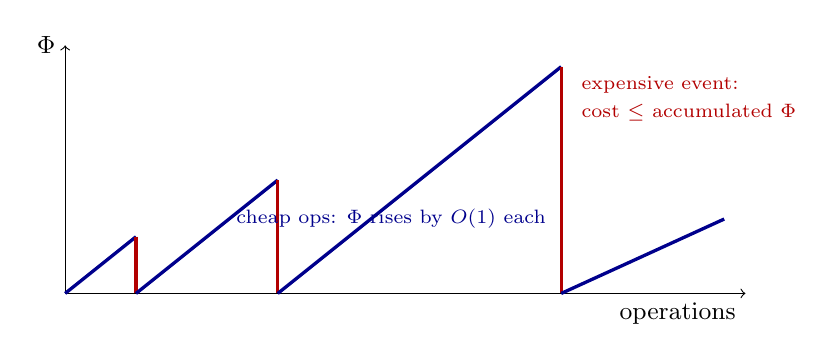
\begin{tikzpicture}[scale=0.9]
  \draw[->] (0,0) -- (9.6,0);
  \node[font=\small, below left] at (9.6,0) {operations};
  \draw[->] (0,0) -- (0,3.5);
  \node[font=\small, left] at (0,3.5) {$\Phi$};
  \draw[very thick, blue!55!black] (0,0) -- (1,0.8);
  \draw[very thick, red!70!black] (1,0.8) -- (1,0);
  \draw[very thick, blue!55!black] (1,0) -- (3,1.6);
  \draw[very thick, red!70!black] (3,1.6) -- (3,0);
  \draw[very thick, blue!55!black] (3,0) -- (7,3.2);
  \draw[very thick, red!70!black] (7,3.2) -- (7,0);
  \draw[very thick, blue!55!black] (7,0) -- (9.3,1.05);
  \node[font=\scriptsize, blue!55!black] at (4.6,1.05)
    {cheap ops: $\Phi$ rises by $O(1)$ each};
  \node[font=\scriptsize, red!70!black, anchor=west] at (7.15,2.95)
    {expensive event:};
  \node[font=\scriptsize, red!70!black, anchor=west] at (7.15,2.55)
    {cost $\le$ accumulated $\Phi$};
\end{tikzpicture}
\caption{The sawtooth: cheap operations deposit into $\Phi$; an expensive
event fires only when enough has accumulated, and its cost is paid entirely
by the drop in $\Phi$. Doubling the event cost doubles the inter-event gap.}
\label{fig:amo-sawtooth}
\end{figure}

The fourth rung packages the aggregate method for periodic structure --- and
it is the form most corpus papers actually use, because a batch schedule is
easier to name than a potential:

\begin{proposition}[Epoch decomposition]\label{prop:amo-epoch}
Partition every execution into consecutive \emph{epochs}, epoch $e$ having
$\mathrm{len}(e)$ operations and total cost $\mathrm{cost}(e)$. Then the
amortized cost per operation is $\sum_e \mathrm{cost}(e) / \sum_e
\mathrm{len}(e)$. In particular, if every epoch costs $O(C)$ and contains at
least $\ell$ operations, the amortized cost is $O(C/\ell)$; if an epoch's
fixed setup $S$ services $T$ operations, its contribution is $O(S/T)$. \eop
\end{proposition}

\begin{proof}
Sum epoch costs, sum epoch lengths, divide; the special cases substitute the uniform bounds.
\end{proof}

\sidenote{Epochs are the aggregate method in periodic clothing, and the
potential method is the accounting method with the balance read off the
state instead of the history; the three proofs are one proof --- sum a
nonnegative quantity --- and the choice is ergonomic: batch schedules state
epochs, accumulation triggers state $\Phi$.}
Sections~\ref{sec:amo-aero} and~\ref{sec:amo-order} below are epoch
arguments; Section~\ref{sec:amo-spline} is a pure potential argument.

\begin{remarkbox}[Notation]
Throughout, $c_i$ is the true cost of operation $i$, $\hat{a}_i$ its amortized
cost, and $\Phi$ a function from states to $\mathbb{R}_{\ge 0}$ with
$\Phi(D_0) = 0$ on the initial state. ``Amortized $O(f)$'' always means
total cost $O(mf)$ for every $m$ and every sequence of $m$ operations from
$D_0$ --- a deterministic statement about worst sequences, with nothing
averaged and nothing probabilistic (per-operation \emph{expected} cost is a
different, randomized contract).
\end{remarkbox}

The price of every rung is the same: the bound is a promise about
\emph{sequences}, not single operations. A deployment needing every request
answered within a deadline requires \emph{deamortized} variants that spread
each burst over neighboring operations \citep{amortized-potential-bg5}.

\subsection{How to choose the method}
\label{sec:amo-choose}

The selection is mechanical once two questions are answered. \emph{First, can
you sum a whole worst-case sequence?} If the total cost of $m$ operations has
a clean combinatorial bound, the aggregate method or its epoch packaging
(Proposition~\ref{prop:amo-epoch}) is the shortest honest proof.
\emph{Second, can you name who pays?} If the expensive event is triggered by
an accumulation you can point at --- rows since the last re-decomposition,
excess of a counter over its budget, rounding slack of a cached value ---
define $\Phi$ on exactly that quantity and verify the three properties of
Theorem~\ref{thm:amo-potential}. Use accounting when the payer is naturally
an operation (``this insert pays for its own future copy''), potential when
it is naturally a state (``every byte above the watermark''), and epochs
whenever the algorithm itself has a batch schedule.

\begin{reachbox}{When to Reach for Amortization}
Reach whenever a component must be certified with a \emph{per-operation}
time or space bound, the algorithm has an occasional expensive structural
event --- split, merge, rebuild, compaction, re-decomposition, full scan ---
and that event only fires after many cheap operations accumulate a trigger:
\begin{enumerate}
\item Identify the expensive rare operation: name the burst, its cost $C$,
  and the measurable quantity that must accumulate before it can fire again.
\item Define the potential on the state: $\Phi$ is that accumulated quantity
  (or the epoch schedule that bounds it), with $\Phi(D_0) = 0$.
\item Charge deposits and withdrawals: every cheap operation raises $\Phi$ by
  at most $O(1)$; every burst drops $\Phi$ by at least its cost $C$ --- so
  the inter-burst gap is $\Omega(C)$ and the amortized cost stays $O(1)$ per
  deposit.
\item Verify $\Phi \ge 0$ initially and throughout: this is what makes the
  telescoping safe for every prefix, and it is the only place amortized
  proofs fail --- one reachable state with $\Phi < 0$ voids the bound.
\end{enumerate}
Caveats before shipping the bound: amortized $\ne$ worst case (budget for
deamortization if tail latency matters), and insertion-only accumulation can
shatter under deletions --- check the fully dynamic lower bounds first.
\end{reachbox}

\section{Enumerating regular pattern matches with amortized constant delay}
\label{sec:amo-enum}

The exemplar is a PODS'26 paper on pattern matching \citep{sigmod26-177}\pods.
Extracting all matches of a \emph{pattern with variables} --- fixed
constants separated by variables standing for arbitrary substrings --- is
the engine behind regex-capture queries, log extraction, and transformation
languages; when the fixed parts are plain strings the pattern is called
\emph{regular}. A match assigns each variable a substring so that the
concatenation equals the text $T$, recorded by the $k$-tuple of positions
where the constants sit. Enumeration algorithms are judged on preprocessing
time, \emph{delay} between outputs, and space; the paper pushes all three to
optimal for this class, including an \emph{amortized} constant-delay
variant and an indexed version answering each later pattern in time
near-linear in the pattern alone --- reported as the first optimal
combined-complexity algorithms for a non-trivial subcase of enumerating
regular-expression matches with capture variables.

\paragraph{Problem.}
Let $T[1..n]$ be a text and $\alpha = w_0 \diamond x_1 w_1 \diamond \dots
\diamond x_k w_{k+1}$ a regular pattern with $\sum_{i=1}^{k} |w_i| \le n$. A
\emph{valid embedding} is a $k$-tuple $(j_1, \dots, j_k)$ such that $w_i$
occurs at position $j_i$ for each $i$, the occurrences are consecutive and
non-overlapping, $w_0$ is a prefix of $T$, and $w_{k+1}$ is the suffix
starting after $j_k + |w_k| - 1$. The task is to enumerate the set $S$ of all
valid embeddings. The difficulty is the output: $|S|$ can reach $n^k$, so
materializing occurrence lists up front risks blowing past $O(n)$, while the
delay must stay constant however the outputs are distributed.

\paragraph{Guarantee.}

\begin{theorem}[Optimal enumeration, Theorems~1.1 and~1.2 of the paper,
notation cleaned]\label{thm:amo-enum}
(i) The set $S$ of all valid embeddings of $\alpha$ in $T$ can be enumerated
with constant delay after preprocessing in $O(n + |S|)$ time, using
$O(n + \min\{|S|, n^k\})$ space. (ii) Alternatively, $S$ can be enumerated
with amortized constant delay after preprocessing in $O(n)$ time and the same
space: for every $s \le |S|$, the first $s$ embeddings are reported in
$O(n + s)$ total time. \eop
\end{theorem}

\sidenote{A third theorem of the paper upgrades to \emph{worst-case}
constant delay with $O(n)$ preprocessing at the price of
$O(n \min\{|S|, n^k\})$ space --- the deamortization trade of
Section~\ref{sec:amo-tool}.}
\paragraph{How amortization is applied.}
The variant (ii) is an aggregate-method argument over the enumeration phase,
and its engine is a counting bound on where embeddings can live. The paper
greedily computes a \emph{left-canonical} embedding $(\ell_1, \dots, \ell_k)$
(each $\ell_i$ the leftmost feasible occurrence of $w_i$) and a symmetric
\emph{right-canonical} embedding $(r_1, \dots, r_k)$; every valid embedding
$(j_i)$ satisfies $\ell_i \le j_i \le r_i$. Write $O_i = \{p \in [\ell_i :
r_i] \mid w_i \text{ occurs at } p\}$; the workhorse is the following bound.

\begin{lemma}[Embedding counting bound, Lemma~3.4 of the paper, notation
cleaned]\label{lem:amo-embed-count}
With $O_i$ and $S$ as above,
$\textstyle\sum_{i=1}^{k} (|O_i| - 1) \le \min\{kn,\ |S|\}$. \eop
\end{lemma}

\begin{proof}[Proof sketch]
$|O_i| \le n$ gives the $kn$ side. For the $|S|$ side, each $j_i \in O_i
\setminus\{\ell_i\}$ substituted into the canonical hybrid yields a valid
embedding, one distinct embedding per pair $(i, j_i)$. (Full proof in
Section~\ref{sec:amo-appendix}.)
\end{proof}

The algorithm runs in two phases. In preprocessing, the intervals
$[\ell_i : r_i + |w_i|)$ are partitioned into \emph{epochs}
(Definition~3.7 of the paper): maximal runs of intervals overlapping
transitively, whose left and right parts are separately pairwise disjoint,
so the total epoch length is $O(n)$. Each epoch is preprocessed
\emph{locally}, in time linear in its length: per-epoch suffix-array and
suffix-tree ranges for the $w_i$ (Lemma~2.2 of the paper), plus a
range-maximum structure enumerating with worst-case constant delay all
suffix-array entries above a threshold (Lemma~2.4). The amortization lives
in the enumeration phase: rather than materializing all lists $O_i$ during
preprocessing (their total length can exceed $n$), the algorithm outputs
the \emph{simple} embeddings --- those differing from the canonical
skeletons in exactly one coordinate --- \emph{while} building the lists,
one output per list element. Lemma~\ref{lem:amo-embed-count} bounds the
simple embeddings by $\min\{kn, |S|\}$, so every unit of
list-materialization work is paid for by an emitted embedding, up to
$O(n + k)$ overhang: the first $s$ embeddings cost $O(n + s)$ total. Once
the lists exist, a radix sort plus constant-delay enumeration (Lemma~3.6)
finishes.

\paragraph{What it buys.}
Preprocessing linear in $n$ \emph{independent of the output size},
amortized constant delay, and space $O(n + \min\{|S|, n^k\})$ --- plus the
indexed variant (each pattern answered in $O(|\alpha| + k \log n)$ plus
constant delay), the shape a database system needs for repeated extraction
queries.

\section[Matrix sketches for streams]{Matrix sketches for streams: batching the re-decomposition}
\label{sec:amo-aero}

The exemplar is a SIGMOD'26 paper on streaming matrix sketches
\citep{sigmod26-015}. A matrix sketch tracks the covariance structure of a
stream of $d$-dimensional row vectors --- the substrate for PCA-style
monitoring, regression, and anomaly detection --- and the standard tool,
Frequent Directions, periodically compresses its summary by an SVD. The
pain: a faithful SVD costs time quadratic in the error parameter, too
expensive to redo on every arrival. The paper proposes AeroSketch, keeping
the same space and error contracts while driving the amortized per-update
time down to what it calls near-optimal, across persistent streams,
sliding windows (only the last $N$ updates matter), and distributed sites
coordinating through a hub. The guarantees hold with tunable high
probability, inherited from iteration error bounds for randomized power
iterations --- and the time bounds are amortized, exactly the
batch-schedule amortization of Proposition~\ref{prop:amo-epoch}.

\paragraph{Problem.}
A stream presents row vectors $a_1, a_2, \dots \in \mathbb{R}^d$ one at a
time; stacking the arrivals so far gives $A$. The sketch $B$ must maintain
the covariance-error guarantee $\| A^{\top} A - B^{\top} B \|_2 \le
\varepsilon \|A\|_F^{2}$, preserving the top of the spectrum. In the
\emph{persistent} setting $A$ is the entire history; in the
\emph{sliding-window} setting only $(T-N, T]$ counts; in the
\emph{distributed} setting $m$ sites observe substreams while a
coordinator keeps the global sketch with bounded communication. The cost
model charges amortized time per update, space, and communication, with
success probability $1 - \delta$ for tunable $\delta$.

\paragraph{Guarantee.}

\begin{theorem}[Tracking matrix sketches, main theorems of the paper,
notation cleaned, $\varepsilon$-dependence restored]
\label{thm:amo-aero}
AeroSketch solves the persistent matrix-sketch tracking problem with space
$O\bigl(\tfrac{d}{\varepsilon} \log \|A\|_F^{2}\bigr)$ and amortized time
$O\bigl(\tfrac{d}{\varepsilon} \log d\bigr)$ per update, with success
probability at least $\tfrac{99}{100}\bigl(1 - \tfrac{2}{\sqrt{e}} \cdot
\tfrac{1}{\sqrt{d \log_2 d}}\bigr)$; with probability amplification it
achieves amortized time $O\bigl(\tfrac{d}{\varepsilon} \log d \log^{2}
\tfrac{1}{\delta}\bigr)$ per update while guaranteeing success probability
at least $1 - \delta$, for tunable $\delta \in (0, 1/100)$; the
sliding-window variant pays an extra $\log R$ in space and amortized
time. \eop
\end{theorem}

\paragraph{How amortization is applied.}
The expensive rare operation is the re-decomposition: when the sketch matrix
$C$ has absorbed $2/\varepsilon$ rows, an eigen-decomposition compresses it
back to $1/\varepsilon$ rows. The paper batches it exactly as in
Proposition~\ref{prop:amo-epoch}:

\begin{lemma}[Batched re-decomposition, Proposition of the paper and its
proof, notation cleaned, $\varepsilon$ restored]\label{lem:amo-aero-batch}
Between two consecutive re-decompositions at least $1/\varepsilon$ updates
elapse (the row count grows by one per update, from $1/\varepsilon$ back up
to $2/\varepsilon$). Each re-decomposition costs $O(d/\varepsilon^{2})$, so
its amortized contribution is $O(d/\varepsilon)$ per update; the per-update
power iteration monitoring the top singular value uses $k = \log_2 d + 1$
steps and costs $O(d \log d)$. Together, the amortized per-update time is
$O\bigl(\tfrac{d}{\varepsilon} \log d\bigr)$. \eop
\end{lemma}

\begin{proof}[Proof sketch]
Rows enter one per update; the decomposition fires exactly when the row count
reaches $2/\varepsilon$ and resets it to $1/\varepsilon$, so every epoch has
length at least $1/\varepsilon$ and one burst of $O(d/\varepsilon^2)$;
divide (full proof in Section~\ref{sec:amo-appendix}).
\end{proof}

The same accounting controls space: a re-decomposition \emph{dumps}
directions $Z_i$ (rank $k_i$) into a snapshot queue, and a dump fires only
after the sketch's residual Frobenius mass above a threshold $\theta$ has
accumulated by $k_i\theta/2$, so the dumped ranks sum to $O(\|A\|_F^2/
\theta)$ --- an implicit potential on the residual mass bounding the
queue. The \emph{whp} part: the re-decomposition only needs its top
singular values approximately; power iteration with $\log_2 d + 1$ steps
fails to halve the top squared singular value with probability at most
$\tfrac{2}{\sqrt{e}} \cdot \tfrac{1}{\sqrt{d \log_2 d}}$ (a corollary in
the paper), which is the success probability of
Theorem~\ref{thm:amo-aero}; amplification repeats the iteration and costs
the $\log^{2}(1/\delta)$ factor. The \emph{composition} part:

\begin{lemma}[Decomposability, Lemma of the paper, notation cleaned]
\label{lem:amo-aero-decomp}
Decompose $A = [A_1, A_2, \dots, A_m]$ into submatrices. If each $B_i$
sketches $A_i$ with covariance error $\|A_i^{\top} A_i - B_i^{\top}
B_i\|_2 \le \varepsilon_i \|A_i\|_F^{2}$, then $B = [B_1, B_2, \dots, B_m]$
sketches $A$ with $\| A^{\top} A - B^{\top} B \|_2 \le
\textstyle\sum_{i=1}^{m} \varepsilon_i \|A_i\|_F^{2}$. \eop
\end{lemma}

\begin{proof}
$A^{\top} A - B^{\top} B = \sum_i (A_i^{\top} A_i - B_i^{\top} B_i)$;
apply the triangle inequality to the spectral norm and substitute each
block's guarantee.
\end{proof}

Sliding windows and distributed sites both become substreams (snapshots are
blocks whose per-block errors add, decomposability summing them), with
communication bounded by the same epoch counting on rounds of a doubling
threshold. The per-update error telescopes over the window: the
accumulated spectral error is the sum of discarded singular values, which
the dump-threshold accounting keeps within $O(\varepsilon)\|A\|_F^2$.

\paragraph{What it buys.}
Amortized $O\bigl(\tfrac{d}{\varepsilon} \log d\bigr)$ per update instead
of an $O(d/\varepsilon^2)$ burst every $\tfrac{1}{\varepsilon}$ updates ---
one proof skeleton covering persistent, sliding-window, and distributed
deployments, with tunable success probability.

\section{Order routing in exchange graphs: epochs over path selections}
\label{sec:amo-order}

The exemplar is a SIGMOD'26 paper on order routing in decentralized finance
\citep{sigmod26-180}. A decentralized exchange is a graph: token pairs are
joined by pools quoting a price (a \emph{weight}) with limited liquidity (a
\emph{capacity}). Routing a market order means repeatedly picking the
cheapest path in this \emph{exchange graph}, executing against it until a
bottleneck capacity is exhausted, re-pricing, and picking again --- and
since every fill moves prices and depletes capacities, the ranking of paths
goes stale after each selection, while re-scanning all candidates after
every fill is quadratic in the path count. The paper builds ORDER, a
path-indexing structure whose maintenance is \emph{lazy} --- cached weights
and capacities refresh only when a correctness invariant demands it ---
certified by an amortized complexity theorem over \emph{epochs} of
selections: contradiction proofs on the global weight ordering prove the
laziness safe, an epoch decomposition proves it cheap.

\paragraph{Problem.}
For each token pair $(u,v)$ an \emph{ordered edge group} $E_g(u,v)$ holds
the parallel edges (feasible swaps) sorted by nondecreasing weight
$w_\ell$, each with capacity $c_\ell$; the \emph{front} of a group is its
minimum-weight edge with remaining capacity. A path $\pi$ carries the
ordering key $W(\pi) = \sum_{g \in \pi} w_g$ (sum of front weights) and
the bottleneck capacity $C(\pi) = \min_{g \in \pi} c_g$. The iterative
selection loop repeatedly extracts the minimum-key path, executes an
amount, consumes capacities along the path (possibly advancing fronts),
and re-ranks. ORDER maintains an \emph{active bucket} --- a heap over the
top-$K$ paths by key --- plus \emph{reserve buckets} holding the remaining
candidates in coarser weight ranges, replenished by periodic rebuilds.

\paragraph{Guarantee.}

\begin{theorem}[Amortized complexity, Theorem~3.9 of the paper, notation
cleaned]\label{thm:amo-order-amort}
Consider the iterative path-selection algorithm over $|P|$ indexed paths
with active-bucket size $K$. One rebuild epoch with $T$ selection
iterations costs $O(|P|) + O(K \log K) + O(T \log K)$, so the amortized
time per selection iteration is $O\bigl(\tfrac{|P|}{T}\bigr) +
O\bigl(\tfrac{K \log K}{T}\bigr) + O(\log K)$. \eop
\end{theorem}

\paragraph{How amortization is applied.}
The proof (transcribed in Section~\ref{sec:amo-appendix}) is a textbook
epoch decomposition in the sense of Proposition~\ref{prop:amo-epoch}: an
epoch is (1)~one scan of all $|P|$ paths recomputing keys and admitting
the top $K$ into the active bucket via a KLL-style quantile sketch, (2)~the
build of that bucket, a heap over at most $K$ paths, and (3)~the $T$
selections, each an extract-min plus a bounded number of localized heap
updates at $O(\log K)$ apiece. The amortization invariant is that the $K$
admitted paths are all consumed \emph{within that same epoch} --- extracted
or evicted --- so the fixed costs (1)--(2) are spread over exactly the $T$
selections they service. What keeps the lazy structure \emph{correct}
while cheap is a pair of contradiction arguments on the ordering of keys:

\begin{lemma}[No-cross-bucket domination, Lemma~4.2 of the paper, notation
cleaned]\label{lem:amo-order-nodom}
Given the prioritized buckets, for any two bucket indices $i < i'$, no path
in $B_{i'}$ has a strictly smaller ordering key than a path in $B_i$:
$\pi_p \in B_i,\ \pi_q \in B_{i'},\ i < i' \Rightarrow W(\pi_p) \le
W(\pi_q)$. \eop
\end{lemma}

\begin{proof}[Proof sketch]
Buckets partition a global sort of paths by $W(\cdot)$ into index-ordered,
non-overlapping ranges; a strict reversal would place $\pi_q$ before $\pi_p$
in that sort, forcing it into a bucket of index at most $i$, contradicting
$\pi_q \in B_{i'}$ with $i' > i$.
\end{proof}

Domination means selection never looks past the active bucket until it is
exhausted; a companion rebuild-truncation lemma shows a rebuild can stop
early while some reserve path is unaffected by recent updates, and an
on-demand bottleneck lemma (Lemma~3.4 of the paper) shows the bottleneck
read off the \emph{current fronts} at selection time already equals the
true one --- so capacities too are maintained lazily, on demand.

\paragraph{What it buys.}
Each fill pays $O(\log K)$-ish maintenance instead of a full re-ranking,
while the routing output remains \emph{exactly} optimal --- laziness
certified safe by the ordering lemmas, not traded against approximation ---
and the epoch schedule says when to expect the next heavier rebuild bill.

\section{Quantile sketches: a potential over bucket counters}
\label{sec:amo-spline}

The exemplar is a SIGMOD'26 paper on quantile sketches \citep{sigmod26-363}.
Estimating quantiles over a stream --- medians, percentiles, heavy
thresholds --- is a core analytics primitive, and the classical
deterministic summaries (GK and its descendants, KLL) share a ceiling:
within a bucket, rank is interpolated under a uniformity assumption, and
that assumption is what their error bounds pay for. SplineSketch instead
interpolates the rank function inside each bucket by a \emph{spline}
(monotone cubic by construction), which tracks skewed data far better;
buckets carry counters, and the sketch stays at $k$ buckets through two
structural events --- a \emph{split} when a counter exceeds its budget and
a \emph{join} of adjacent buckets to reclaim space. The analysis questions
are exactly amortization questions --- how many splits can a stream force,
and how much rank error does each deposit? --- answered by an explicit
potential over the bucket counters, the purest $\Phi$-argument in this
chapter's corpus.

\paragraph{Problem.}
A stream of $n$ items arrives; the sketch keeps $k$ buckets over the value
range, bucket $i$ being an interval $(\sigma_{i-1}, \sigma_i]$ between
thresholds with a counter $b_i$ of absorbed items. Arrivals are buffered
and periodically merged into buckets; to keep at most $k$ buckets, a bucket
violating the \emph{bucket bound} $b_i \le C_b \cdot n/k$ must \emph{split},
and adjacent buckets are \emph{joined} to reclaim space --- a pair is
\emph{joinable} if the merged counter satisfies $b_i + b_{i+1} \le 0.75
\cdot C_b \cdot n/k$ and the threshold $\sigma_i$ is not \emph{protected}
(freshly created by a split). Queries are answered by the counters plus
spline interpolation inside each bucket. The task is to bound the number
of splits --- hence the protected thresholds, hence the ability to always
find a joinable pair --- and the resulting rank error.

\paragraph{Guarantee.}

\begin{theorem}[Rank error, from the paper's error analysis, notation
cleaned]\label{thm:amo-spline-error}
After processing $n$ items (with a Misra--Gries sketch of size $O(k)$
filtering heavy hitters in parallel), for any threshold $\sigma_i$ of the
final sketch the rank error obeys
\[
\varepsilon^{n}(\sigma_i) \;\le\; O\bigl(\log \alpha \cdot n/k\bigr),
\]
where $\alpha$ is the paper's aspect-ratio parameter of the stream; the
lower error is symmetric, and in the mergeable setting the bound is
$O\bigl(\log (n/k) \cdot n/k\bigr)$. \eop
\end{theorem}

\paragraph{How amortization is applied.}
Nothing here is random --- this is deterministic bookkeeping. The paper
defines the potential of a sketch state $S$ at time $t''$ with $k(S)$ buckets
as the total \emph{excess of the counters over the join budget}:
\[
\Phi(S) \;=\; \textstyle\sum_{i=1}^{k(S)} \max\Bigl\{\,0,\;
b_i - 0.75 \cdot C_b \cdot t''/k \,\Bigr\},
\]
and verifies exactly the reachbox recipe: $\Phi(S) \in [0, t'']$
(nonnegativity); each of the $t - t'$ arrivals in an interval $(t', t]$
increments one counter by one, raising $\Phi$ by at most $1$ (deposits,
total increase $\le t - t'$); joins never raise $\Phi$ (joinability keeps
the merged counter at or below the join budget, where the max-terms
vanish); and every forced split \emph{decreases} $\Phi$ by at least
$\beta \cdot C_b \cdot t / (2.5 k)$ for a placement constant $\beta$
(withdrawals). The workhorse is then pure division:

\begin{lemma}[Split budget, from the paper's analysis, notation cleaned]
\label{lem:amo-spline-split}
The number of splits during $(t', t]$ is at most
$\frac{t - t'}{\beta C_b t / (2.5 k)} = \frac{2.5\,k}{\beta C_b} \le
\frac{k}{18}$, with $C_b$ chosen as a function of $\beta$. \eop
\end{lemma}

\begin{proof}[Proof sketch]
Divide the total possible deposit $t - t'$ by the minimum withdrawal per
split; the withdrawal case analysis is in Section~\ref{sec:amo-appendix}.
\end{proof}

The split budget powers two conclusions. First, protected thresholds are
bounded (each split creates $O(1)$), so a counting argument shows the
sketch \emph{always} contains a joinable pair --- too many unjoinable
adjacent pairs would need more protected thresholds than splits can create
or more counter mass than $t$ items supply. Second, the rank error is
\emph{charged along the split history}: a threshold's error grows only at
splits, and each ancestor in the merge tree contributes a geometrically
shrinking share --- the same arithmetic in log scale, giving the
$O(\log \alpha \cdot n/k)$ bound. The spline itself contributes a
feasibility lemma proved by a coefficient argument:

\begin{lemma}[Spline midpoint bound, Lemma of the paper, notation cleaned]
\label{lem:amo-spline-midpoint}
Let $P(x)$ be a cubic polynomial with $P(0) = 0$, $P(1) = 1$, non-decreasing
on $[0,1]$. Then $P(\tfrac12) \in [\beta,\, 1 - \beta]$ with
$\beta = \tfrac12 - \tfrac{\sqrt{3}}{4} \approx 0.067$. \eop
\end{lemma}

\begin{proof}[Proof sketch]
Write $P(\lambda) = a\lambda^3 + b\lambda^2 + c\lambda$ with $a + b + c =
1$; monotonicity forces $3a\lambda^2 + 2b\lambda + c \ge 0$ on $[0,1]$, and
evaluating that constraint at one well-chosen test point bounds
$-(\tfrac{3a}{8} + \tfrac{b}{4})$, which is exactly $\tfrac12 -
P(\tfrac12)$. (Full proof, with the test point, in
Section~\ref{sec:amo-appendix}.)
\end{proof}

The lemma guarantees the interpolation inside any bucket is never
arbitrarily skewed at its midpoint --- the coefficient feasibility that
makes the spline's error arithmetic work with clean constants.

\paragraph{What it buys.}
$O(\log k)$ per operation via two heaps and a queue, deterministic and
mergeable with the stated error guarantees, and --- the experimental
headline --- noticeably more accurate quantiles than KLL and GK-style
baselines at equal space, because the potential certifies a thrifty split
schedule.

\section{Advanced usage and further reading}
\label{sec:amo-advanced}

The two usages sketched here compose the tool with other theory: an
amortized bound purchased at the price of approximation, certified
unavoidable by a lower-bound reduction; and an amortized update bound
riding a DP space optimization.

\paragraph{Approximate query processing under updates
\citep{sigmod26-274}.}
Maintaining the answer to a conjunctive query over a semiring under updates
is blocked, outside the tiny q-hierarchical class, by dynamic lower bounds:
any non-q-hierarchical Boolean CQ needs amortized $\Omega(\sqrt{N})$ update
time under fully dynamic sequences. The paper's escape splits the
free-connex join tree into an \emph{exact connex part} (helper views kept
exact, so enumeration stays constant-delay) and an \emph{approximated
part}, whose cached annotations are rounded to a factor $b$ and refreshed
lazily when the true value outgrows the cache. The potential is the total
rounding slack: an insertion deposits $O(1)$, a recomputation cascade fires
only when some tuple's slack is exhausted, and each tuple can fire at most
$\log_b M$ times, $M$ the largest annotation ever cached. The guarantee
(Theorem~4.7 of the paper): for any $b > 1$ and free-connex query, all
auxiliary views update in amortized $O(\log_b M)$ time under
insertion-only sequences (for the join size of a 3-way join, $O(\log_b
N)$). The hypothesis is necessary: any multiplicative approximation on the
semiring $(\mathbb{R}_{\ge 0}, +, \times)$ yields exact answers on the
Boolean semiring, so the $\Omega(\sqrt{N})$ fully-dynamic lower bound
transfers.

\paragraph{RadixGraph: amortized compaction over log segments
\citep{sigmod26-203}.}
RadixGraph is a dynamic graph storage structure: adjacency is compressed
into radix-tree layers over bit prefixes of vertex ids, and updates append
to log segments periodically \emph{compacted} back into the layers. The
layer structure is chosen by an occupancy model whose space objective is
minimized by a DP over layer splits, computable in $O(nlx^{2})$ time and
$O(lx)$ space. On top sits the amortized bound (Theorem and proof sketch
of the paper): edge insertion, update, and deletion cost amortized $O(1)$
--- appending to a non-full log segment costs $O(1)$, and when a segment
fills, the compaction costs $O(d)$ but is charged to the $\Omega(d)$
appends that must accumulate before it can fire, epoch counting in its
barest form.

\subsection{Further reading}

\begin{itemize}
\item The amortized-analysis chapters of Cormen et al.\
\citep{amortized-potential-bg3} --- aggregate, accounting, and potential
methods with the dynamic-table example.
\item Tarjan's survey \citep{amortized-potential-bg1}, with the union--find
and splay-tree classics \citep{amortized-potential-bg2}.
\item Overmars \citep{amortized-potential-bg5} --- periodic rebuilding as
the degenerate epoch schedule, and the deamortization caveats.
\item Greenwald and Khanna \citep{amortized-potential-bg4} --- quantile
summaries where potential-bounded compaction first appeared in the DB
literature; the ancestor of Section~\ref{sec:amo-spline}'s analysis.
\end{itemize}

\begin{recap}
\item \textbf{What the tool is.} Amortized analysis certifies per-operation
  time/space bounds over \emph{sequences}: bursts are rare because they
  require accumulation, and the certificate is a bank balance (accounting),
  a state function $\Phi \ge 0$ (potential), or a batch schedule (epochs).
\item \textbf{Which rung when.} Clean global sum of a worst-case sequence:
  aggregate. Explicit batch schedule (re-decompose every $\ell$ arrivals,
  rebuild after $T$ selections): epoch decomposition
  (Proposition~\ref{prop:amo-epoch}). Measurable state trigger (counter
  excess, rounding slack, residual mass): potential
  (Theorem~\ref{thm:amo-potential}). Payer naturally an operation:
  accounting (Theorem~\ref{thm:amo-accounting}).
\item \textbf{Why it works.} Telescoping: $\sum_i c_i = \sum_i \hat{a}_i -
  \Phi(D_m) \le \sum_i \hat{a}_i$ whenever $\Phi \ge 0$ and $\Phi(D_0) = 0$;
  the failure modes are a reachable state with $\Phi < 0$, or a burst that
  fires without its accumulation.
\item \textbf{What the corpus showed.} Pattern enumeration
  (Section~\ref{sec:amo-enum}): a counting bound pays for list
  materialization with outputs --- amortized $O(1)$ delay. Matrix sketches
  (Section~\ref{sec:amo-aero}): SVD bursts batched over $1/\varepsilon$
  arrivals, composed across windows and sites. Order routing
  (Section~\ref{sec:amo-order}): rebuild epochs over $T$ selections,
  contradiction proofs certifying lazy maintenance. Quantile sketches
  (Section~\ref{sec:amo-spline}): a potential over bucket counters bounds
  splits by $k/18$; rank error is charged along the split history.
\item \textbf{Advanced usage.} Amortization purchased with approximation
  ($O(\log_b M)$ updates at factor-$b$ rounding, lower bound imported by a
  Boolean-semiring reduction), and amortized $O(1)$ graph updates riding a
  DP-optimal layout (Section~\ref{sec:amo-advanced}). Deferred proofs are
  collected in the Appendix (Section~\ref{sec:amo-appendix}).
\end{recap}

\section{Appendix}
\label{sec:amo-appendix}

Proofs omitted from the main text are collected here.

\subsubsection*{Proof of Lemma~\ref{lem:amo-embed-count} (embedding counting)}
{\itshape Statement (recalled).} For the valid occurrence sets $O_i \subseteq
[\ell_i : r_i]$ of the constant strings $w_i$ and the set $S$ of all valid
embeddings, $\sum_{i=1}^{k} (|O_i| - 1) \le \min\{kn, |S|\}$.\eop

\begin{proof}
The bound $\sum_i (|O_i| - 1) \le kn$ is immediate from $|O_i| \le n$. For
the second bound, the paper's canonical-embedding lemma gives that for
$j_i \in O_i \setminus\{\ell_i\}$ the hybrid tuple $(\ell_1, \dots,
\ell_{i-1},\, j_i,\, r_{i+1}, \dots, r_k)$ is a valid embedding: anchoring
the prefix at the leftmost and the suffix at the rightmost feasible
occurrences leaves every intermediate valid occurrence of $w_i$ feasible.
So each $i$ yields $|O_i| - 1$ valid embeddings, pairwise distinct --- two
for the same $i$ differ in coordinate $i$, and two for $i_1 < i_2$ differ in
coordinate $i_1$. All lie in $S$, so $\sum_i (|O_i| - 1) \le |S|$.
\end{proof}

\subsubsection*{Proof of Lemma~\ref{lem:amo-aero-batch} (batched
re-decomposition)}
{\itshape Statement (recalled).} Re-decompositions fire at most once per
$1/\varepsilon$ updates, each costs $O(d/\varepsilon^{2})$, and the
per-update power iteration costs $O(d \log d)$; the amortized per-update
time is $O\bigl(\tfrac{d}{\varepsilon} \log d\bigr)$.\eop

\begin{proof}
The sketch matrix $C$ gains one row per update; the re-decomposition
triggers when the row count reaches $2/\varepsilon$ and resets it to
$1/\varepsilon$, so consecutive triggers are at least $\tfrac{1}{\varepsilon}$
updates apart --- epochs of Proposition~\ref{prop:amo-epoch} with
$\ell = 1/\varepsilon$. The trigger costs the eigen-decomposition of a
$d \times \tfrac{2}{\varepsilon}$ matrix, $O(d/\varepsilon^{2})$ in the
paper's accounting, an amortized $O(d/\varepsilon)$ per update.
Independently, every update runs a power iteration with $k = \log_2 d + 1$
matrix--vector products, $O(d\log d)$, against the dump threshold. Since
$d \log d \le \tfrac{d}{\varepsilon} \log d$ for $\varepsilon \le 1$, the
contributions sum to $O\bigl(\tfrac{d}{\varepsilon} \log d\bigr)$
amortized per update.
\end{proof}

\subsubsection*{Proof of Theorem~\ref{thm:amo-order-amort} (epoch accounting)}
{\itshape Statement (recalled).} One rebuild epoch with $T$ selections costs
$O(|P|) + O(K \log K) + O(T \log K)$, so the amortized time per selection is
$O\bigl(\tfrac{|P|}{T}\bigr) + O\bigl(\tfrac{K \log K}{T}\bigr) +
O(\log K)$.\eop

\begin{proof}
Decompose the epoch as in the paper's proof. (1) \emph{Scan and admission},
$O(|P|)$: all $|P|$ paths are visited once to recompute weights and assign
reserve-bucket ranges; the top $K$ are selected through a KLL-style
quantile sketch, which returns the admission threshold and emits the top
$K$ items. (2) \emph{Active-bucket build}, $O(K \log K)$: a binary heap
over at most $K$ paths. (3) \emph{Per-selection maintenance},
$O(T \log K)$: each selection is one extract-min plus $O(1)$ localized
heap updates at $O(\log K)$ each. The amortization invariant --- every
path admitted in (1) is consumed within the same epoch --- ensures the
fixed costs (1)--(2) are covered by exactly the $T$ selections they
service; summing and dividing by $T$ (Proposition~\ref{prop:amo-epoch})
yields the per-iteration bound.
\end{proof}

\subsubsection*{Proof of Lemma~\ref{lem:amo-spline-split} (split budget)}
{\itshape Statement (recalled).} With
$\Phi(S) = \sum_{i=1}^{k(S)} \max\{0, b_i - 0.75 \cdot C_b \cdot t''/k\}$,
the number of splits during $(t', t]$ is at most
$\tfrac{2.5 k}{\beta C_b} \le \tfrac{k}{18}$.\eop

\begin{proof}
Write $\tau_J = 0.75 \cdot C_b \cdot t''/k$ for the join budget at time
$t''$. \emph{Deposits:} each of the $t - t'$ arrivals increments one
counter by one, so $\Phi$ rises by at most $1$ per arrival (total increase
$\le t - t'$), and $\Phi \ge 0$ throughout since every summand is
nonnegative. \emph{Joins:} joinability gives $b_i + b_{i+1} \le \tau_J$,
so the pre-join summands and the post-join one vanish; joins never
increase $\Phi$. \emph{Withdrawals:} a split at time $t'' \in (t', t]$
fires on a bucket with $b_i > C_b t''/k$, whose summand contributes
$b_i - \tau_J > 0.25\,C_b t''/k$; the split places the new threshold so
each child receives at least a $\beta$-fraction of the parent's counter
($2.5 = 1/\beta$). If both children have counters $\ge \tau_J$, the
decrease is exactly $\tau_J \ge 0.75\,C_b t''/k$; otherwise the smaller
child's summand vanishes and the decrease is at least that counter,
$\ge \beta b_i > \beta C_b t''/k \ge \beta C_b t/(2.5k)$ (using
$t'' \le t$) --- the paper's uniform withdrawal, met in both cases.
\emph{Division:} total decrease cannot exceed total increase, so splits
number at most $\frac{t - t'}{\beta C_b t/(2.5k)} = \frac{2.5k}{\beta C_b}
\le k/18$, by the paper's calibration of $C_b$ from $\beta$.
\end{proof}

\subsubsection*{Proof of Lemma~\ref{lem:amo-spline-midpoint} (spline
midpoint)}
{\itshape Statement (recalled).} If $P$ is cubic with $P(0) = 0$, $P(1) = 1$,
non-decreasing on $[0,1]$, then $P(\tfrac12) \in
[\tfrac12 - \tfrac{\sqrt3}{4},\, \tfrac12 + \tfrac{\sqrt3}{4}]$.\eop

\begin{proof}
By symmetry ($Q(x) = 1 - P(1-x)$ is again cubic, non-decreasing, with
$Q(\tfrac12) = 1 - P(\tfrac12)$) it suffices to prove
$P(\tfrac12) \le \tfrac12 + \tfrac{\sqrt{3}}{4}$. Write
$P(\lambda) = a\lambda^{3} + b\lambda^{2} + c\lambda$: $P(1) = 1$ gives
$a + b + c = 1$, and monotonicity gives $P'(\lambda) = 3a\lambda^{2} +
2b\lambda + c \ge 0$ on $[0,1]$. Since $P(\tfrac12) = \tfrac12 -
(\tfrac{3a}{8} + \tfrac{b}{4})$, it remains to bound
$-(\tfrac{3a}{8} + \tfrac{b}{4})$. Substituting $c = 1 - a - b$ into the
derivative constraint and evaluating at the test point $\lambda^{*} =
\tfrac{3+\sqrt{3}}{6} \in [0,1]$, where $3\lambda^{*2} - 1 =
\tfrac{\sqrt{3}}{2}$ and $2\lambda^{*} - 1 = \tfrac{\sqrt{3}}{3}$, yields
\[
0 \;\le\; (3\lambda^{*2} - 1)\,a + (2\lambda^{*} - 1)\,b + 1
\;=\; \sqrt{3}\Bigl(\tfrac{a}{2} + \tfrac{b}{3}\Bigr) + 1,
\]
so $\tfrac{a}{2} + \tfrac{b}{3} \ge -\tfrac{1}{\sqrt{3}}$; multiplying by
$-\tfrac34$ gives $-(\tfrac{3a}{8} + \tfrac{b}{4}) \le
\tfrac{3}{4\sqrt{3}} = \tfrac{\sqrt{3}}{4}$, hence the claim by symmetry.
\end{proof}

\bibliographystyle{plainnat}
\bibliography{chapters/amortized-potential-all}
